\section{Constructing an effective model}

Before reviewing the algorithm, we present two examples on how to use Pymablock
to find effective models for a k.p model and a tight-binding system, with the
purpose of illustrating the package's capabilities with symbolic Hamiltonian,
large Hilbert spaces and high orders.

\subsection{Pymablock workflow}

\co{The workflow of Pymablock consists of three steps.}
Building an effective model using Pymablock is a three step process:
%
\begin{itemize}
\item Define a Hamiltonian
\item Call \mintinline{python}|pymablock.block_diagonalize|
\item Request the desired order of the effective Hamiltonian
\end{itemize}
%
The following code snippet shows how to use Pymablock to compute the fourth
order correction to an effective Hamiltonian $\tilde{\mathcal{H}}$:
%
\begin{minted}{ipython}
# Define perturbation theory
H_tilde, *_ = block_diagonalize([H_0, H_1], subspace_eigenvectors=[vecs_A, vecs_B])

# Request 4th order correction to the effective Hamiltonian
H_AA_4 = H_tilde[0, 0, 4]
\end{minted}

\co{Depending on the input Hamiltonian, Pymablock uses specific routines to find
the effective model, so that symbolic expressions are compact and numerics are
efficient.}

The function \mintinline{python}|block_diagonalize| interprets the Hamiltonian
$H_0 + H_1$ as a series with two terms, zeroth and first order, and calls the
block diagonalization routine.
This is the main function of Pymablock, and it is the only one that the user
ever needs to call.
Its first output is a multivariate series whose terms are different blocks and
orders of the transformed Hamiltonian.
Calling \mintinline{python}|block_diagonalize| does not compute the series
elements, so the cost of the call is a constant overhead.

\subsection{k.p model of bilayer graphene}

\co{We use bilayer graphene to illustrate how to use Pymablock with analytic models.}

To illustrate how to use Pymablock with analytic models, we consider two layers
of graphene stacked on top of each other.
Our goal is to find the low energy model near the $\mathbf{K}$ point
\cite{McCann_2013}.
First, we construct the Hamiltonian of bilayer graphene from its tight-binding
model.
%
\begin{figure}[!htbp]
\centering
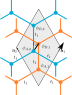
\includegraphics[width=0.3125\linewidth]{figures/bilayer.pdf}
\caption[]{Crystal structure and hoppings of bilayer graphene.}
\label{fig:bilayer}
\end{figure}
%
The main features of the model are its 4-atom unit cell spanned by vectors
$\mathbf{a}_1 = (1/2, \sqrt{3}/2)$ and $\mathbf{a}_2=( -1/2, \sqrt{3}/2)$,
and with wave functions $\phi_{A,1}, \phi_{B,1}, \phi_{A,2}, \phi_{B,2}$.
The model has hoppings $t_1$ and $t_2$ within and between the layers,
respectively, as shown in Fig.~\ref{fig:bilayer}.
We also include an onsite potential $\pm m$ in each layer, such that the
Hamiltonian is gapped, a requirement for perturbation theory to be valid.

We define the Bloch Hamiltonian using the Sympy package for symbolic Python
\cite{Meurer_2017}.
%
\begin{minted}{ipython}
t_1, t_2, m = sympy.symbols("t_1 t_2 m", real=True)
alpha = sympy.symbols(r"\alpha")

H = Matrix([
    [m, t_1 * alpha, 0, 0],
    [t_1 * alpha.conjugate(), m, t_2, 0],
    [0, t_2, -m, t_1 * alpha],
    [0, 0, t_1 * alpha.conjugate(), -m]]
)
\end{minted}

$$
H =
\begin{pmatrix}
m & t_1 \alpha & 0 & 0\\
t_1 \alpha^{*} & m & t_2 & 0\\
0 & t_2 & -m & t_1 \alpha\\
0 & 0 & t_1 \alpha^{*} & -m
\end{pmatrix}
$$
%
where $\alpha(\mathbf{k}) = 1 + e^{i \mathbf{k'} \cdot (\mathbf{a}_1 +
\mathbf{a}_2)}$ and $\mathbf{k'} = (4\pi/3 + k_x, k_y)$, such that
$\alpha(\mathbf{K}) = 0$ and $\mathbf{K}=(4\pi/3, 0)$ is the reference point
for the k.p effective model.
In addition, we use $m$ as a perturbative parameter to demonstrate Pymablock's
capabilities with several perturbations.

\co{We define the perturbative series}
To call \mintinline{python}|block_diagonalize|, we need to define the subspaces
for the block diagonalization, so we compute the eigenvectors of the
unperturbed Hamiltonian at the $\mathbf{K}$ point, $H(\alpha(\mathbf{K}) = m =
0)$.
This operation is a one-time cost, and due to the sparsity of $H_0$, computing
\mintinline{Python}|vecs| is fast.
Then, we substitute $\alpha(\mathbf{k})$ into the Hamiltonian, and define the
block diagonalization routine using that $k_x$, $k_y$, and $m$ are perturbative
parameters via the \mintinline{Python}|symbols| argument.
%
\begin{minted}{ipython}
vecs = H.subs({alpha: 0, m: 0}).diagonalize(normalize=True)[0]

H_tilde, U, U_adjoint = block_diagonalize(
    H.subs({alpha: alpha_k}),
    symbols=(k_x, k_y, m),
    subspace_eigenvectors=[vecs[:, :2], vecs[:, 2:]]
)
\end{minted}
%
The order of the variables in the perturbative series will be that of
\mintinline{python}{symbols}.
For example, requesting the first order term in $k_x$ and $k_y$ from the
effective model is done by calling \mintinline{python}|H_tilde[0, 0, 1, 1, 0]|,
where the first two indices are the block indices (AA), and the next four are
the powers of $k_x$, $k_y$, and $m$, respectively.
We need corrections up to third order in momentum to compute the standard
quadratic dispersion of bilayer graphene and trigonal warping.
We query these terms from \mintinline{Python}|H_tilde| and those proportional
to mass to obtain the effective Hamiltonian:
%
{\small
\begin{gather}
\mathcal{H}^{AA} =
\begin{pmatrix}
m & \frac{3 t_1^2}{4 t_2} ( - k_x^2 - 2ik_x k_y + k_y^2) \\
\frac{3 t_1^2}{4 t_2} ( - k_x^2 + 2ik_x k_y + k_y^2) & -m
\end{pmatrix} + \nonumber \\
\begin{pmatrix}
\frac{3 m t_1^2}{2 t_2^2} ( - k_x^2 - k_y^2) & \frac{\sqrt{3} t_1^2}{8 t_2} (k_x^3 - 5ik_x^2 k_y + 9 k_x k_y^2 + 3ik_y^3) \\
\frac{\sqrt{3} t_1^2}{8 t_2} (k_x^3 + 5ik_x^2 k_y + 9 k_x k_y^2 - 3ik_y^3) & \frac{3 m t_1^2}{2 t_2^2} (k_x^2 + k_y^2)
\end{pmatrix} \nonumber
+
\mathcal{O}(k^4, m^2)
\end{gather}
}
%
The first term contains the standard quadratic dispersion of bilayer graphene
with a gap.
The second term contains trigonal warping and the coupling between the gap and
momentum.
All the terms take less than two seconds in a personal computer to compute.

\subsection{Induced gap in a double quantum dot}

\co{Large systems pose an additional challenge due to the scaling of linear
algebra routines for large matrices.}
Large systems pose an additional challenge due to the cubic scaling of linear
algebra routines on matrices' size.
To overcome this, Pymablock is equipped with an implicit method, which uses
sparse arrays and avoids the construction of the full Hamiltonian.
We illustrate its efficiency with a model of two quantum dots coupled to a
superconductor between them.

\co{We use Kwant to build the Hamiltonian of the system.}
We use the Kwant package \cite{Groth_2014} to build the Hamiltonian of the
system.
In the following code, we define a square lattice of $L \times W = 200 \times
40$ sites with 2 orbitals per unit cell, shown in Fig.~\ref{fig:QD_lattice}.
The lattice is divided into three regions: a quantum dot on the left, a
superconducting region in the middle, and a quantum dot on the right.
%
\inputminted[firstline=15, lastline=48]{ipython}{code_figures/lattice_system.py}
%
The chemical potentials of the normal and superconducting regions are $\mu_n$
and $\mu_{sc}$, respectively, $\Delta$ is the superconducting gap, and $t$
is the hopping amplitude within each region.
The barrier strength between the quantum dots and the superconductor is
$t_{barrier}$, a parameter that we treat as a perturbation.
We will also consider the asymmetry of the dot potentials, $\delta \mu$, as a
perturbation.
%

The system is large: with this many sites even storing all the eigenvectors
would take 60 GB of memory.
Therefore, we use sparse matrices and compute only a few eigenvectors.
In this case, perturbation theory allows us to compute the effective
Hamiltonian of the low energy degrees of freedom only.
To get the unperturbed Hamiltonian, we use the following values for $\mu_n$,
$\mu_{sc}$, $\Delta$, $t$, and $t_{\text{barrier}}$.
%
\inputminted[firstline=50, lastline=51]{ipython}{code_figures/lattice_system.py}
%
The barrier strength and the asymmetry of the dot potentials are the two
perturbations that we vary.
%
\inputminted[firstline=53, lastline=58]{ipython}{code_figures/lattice_system.py}

Since the Hamiltonian is large and we are only interested in the low energy
subspace, it is sufficient to compute the 4 lowest orthonormal eigenvectors of
the unperturbed Hamiltonian.
These are the lowest energy Andreev states in the two quantum dots.
%
\inputminted[firstline=60, lastline=61]{ipython}{code_figures/lattice_system.py}
%
We now define the block diagonalization routine using the implicit method,
which we call by providing the set of vectors of the interesting subspace only.
%
\inputminted[firstline=63, lastline=63]{ipython}{code_figures/lattice_system.py}
%
Block diagonalization is now the most time consuming step because it requires
pre-computing several decompositions of the full Hamiltonian.
It is, however, manageable and it only produces a constant overhead.

To compute the spectrum, we collect the lowest three orders in each parameter
in an appropriately sized tensor.
%
\inputminted[firstline=65, lastline=68]{ipython}{code_figures/lattice_system.py}
%
This takes a few seconds to compute, and we can now compute the low energy
spectrum after rescaling the perturbative corrections by the magnitude of each
perturbation.
%
\inputminted[firstline=71, lastline=76]{ipython}{code_figures/lattice_system.py}
%
Finally, we plot the spectrum.
%
\begin{figure}[h!]
\centering
\includegraphics[width=\linewidth]{figures/lattice_system.pdf}
\caption{Low energy spectrum of the double quantum dot system.
\todo[inline]{Fix ticks.}
}
\label{fig:QD_spectrum}
\end{figure}
%
As expected, the crossing at $E=0$ due to the dot asymmetry is lifted when the
dots are coupled to the superconductor.
In addition, we observe how the proximity gap of the dots increases with the
coupling strength.

In this example the total runtime of Pymablock would only allow us to compute
the spectrum at around 3 points in the parameter space.
This is demonstrates the speed of the implicit method and the efficiency of
Pymablock's algorithm.
